\documentclass[tikz,border=2pt]{standalone}
\usepackage{amsmath,amssymb}
\usetikzlibrary{positioning,calc}
\begin{document}
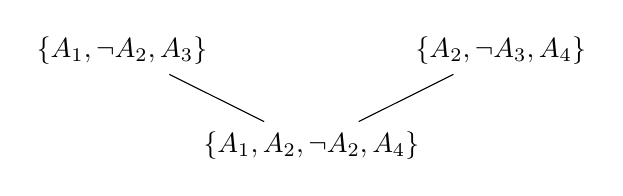
\begin{tikzpicture}
    \node (c1) {$\{A_1,\neg A_2,A_3\}$};
    \node (c2) [right=2.4cm of c1] {$\{A_2,\neg A_3,A_4\}$};
    \node (r) [below=0.9cm of $(c1)!0.5!(c2)$] {$\{A_1,A_2,\neg A_2,A_4\}$};
    \draw (c1) -- (r);
    \draw (c2) -- (r);
\end{tikzpicture}
\end{document}
